\section{逗号运算符}
\begin{frame}[fragile]\ft{\secname}
  逗号运算符扩展了for循环的灵活性,它使你可以在一个for循环中使用多个初始化或更新表达式。
\end{frame}

\begin{frame}[fragile]\ft{\secname}
  \begin{biancheng}
    打印一类邮资费率。费用标准为:第1盎司为37美分,然后每增加1盎司费用增加23美分。
  \end{biancheng}
\end{frame}

\begin{frame}[fragile]\ft{\secname}
  \lstinputlisting[numbers=left]{ch06/code/postage.c}    
\end{frame}

\begin{frame}[fragile]\ft{\secname}
\begin{lstlisting}[backgroundcolor=\color{red!10}]
 1 $0.37
 2 $0.60
 3 $0.83
  ...
\end{lstlisting}
\end{frame}


\begin{frame}[fragile]\ft{\secname}
\begin{figure}
\centering
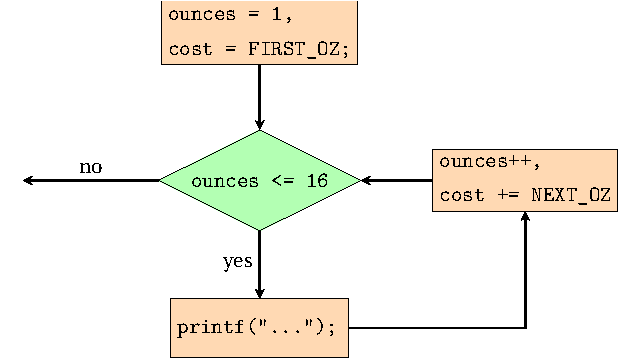
\includegraphics[width=4in]{ch06/images/flowchart.pdf}
\end{figure}

\end{frame}


\begin{frame}[fragile]\ft{\secname}
\begin{itemize}
\item
 逗号运算符并不只限于在for循环中使用,但在for循环中最常使用。
\end{itemize}
\end{frame}


\begin{frame}[fragile]\ft{\secname}
\begin{itemize}
\item
  逗号运算符保证被它分开的表达式按从左到右的次序进行计算。
  \vspace{.1in}
  
  也就是说,逗号是个顺序点,逗号左边的副作用会在程序运行到逗号右边之前生效。
\begin{lstlisting}
ounces++, cost = ounces * FIRST_OZ
\end{lstlisting}
\end{itemize}

\end{frame}

\begin{frame}[fragile]\ft{\secname}
\begin{itemize}
\item
整个逗号表达式的值是右边成员的值。
\begin{lstlisting}
x = (y = 3, (z = ++y + 2) + 5);
\end{lstlisting}
的效果是
\begin{lstlisting}
(1) y = 3;
(2) y = y + 1 = 4;
(3) z = (y + 2) = (4 + 2) = 6;
(4) x = z + 5 = 6 + 5 = 11;
\end{lstlisting}
\end{itemize}

\end{frame}

\begin{frame}[fragile]\ft{\secname}
\begin{lstlisting}
houseprice = 249,500;
\end{lstlisting}
等效于
\begin{lstlisting}
houseprice = 249;
500;
\end{lstlisting}
\pause\vspace{0.1in}

C把它解释为一个逗号表达式,\lstinline|houseprice = 249| 为左子表达式,而 \lstinline|500| 为右子表达式。因此整个逗号表达式的值为右子表达式的值 \lstinline|500|,而左子表达式将变量 \lstinline|houseprice| 赋值为 \lstinline|249|。

\end{frame}

\begin{frame}[fragile]\ft{\secname}
\begin{lstlisting}
houseprice = (249,500);
\end{lstlisting}
\pause\vspace{0.1in}

把右子表达式的值500赋给变量houseprice。
\end{frame}

\begin{frame}[fragile]\ft{\secname}
逗号也用作分隔符。
\begin{lstlisting}
int m, n;
printf("%d %d\n", m, n);
\end{lstlisting}
\pause\vspace{0.1in}

这里,逗号都是分隔符,而不是逗号运算符。
\end{frame}

\begin{frame}[fragile]\ft{\secname}
\begin{li}
计算
$$
S = 1 + \frac12 + \frac14 + \frac18 + \frac1{16} +\cdots 
$$
\end{li}
\end{frame}

\begin{frame}[fragile,allowframebreaks]\ft{\secname}
\lstinputlisting[numbers=left]{ch06/code/zeno.c}
\end{frame}

\begin{frame}[fragile]\ft{\secname}
 \begin{lstlisting}[backgroundcolor=\color{red!10}]
Enter the number of terms you want: 10
sum = 1.000000 when terms = 1.
sum = 1.500000 when terms = 2.
sum = 1.750000 when terms = 3.
sum = 1.875000 when terms = 4.
sum = 1.937500 when terms = 5.
sum = 1.968750 when terms = 6.
sum = 1.984375 when terms = 7.
sum = 1.992188 when terms = 8.
sum = 1.996094 when terms = 9.
sum = 1.998047 when terms = 10.
\end{lstlisting}
\end{frame}
